% Kuber: Geometry-General Neural Surrogates for Conjugate Heat Transfer
% IEEE conference (ICRA) format. Compiles with pdflatex or on Overleaf.
% Requires the IEEEtran class (standard on Overleaf). Figures in ../assets/sim/.
\documentclass[conference]{IEEEtran}
\IEEEoverridecommandlockouts
\usepackage{cite}
\usepackage{graphicx}
\usepackage{booktabs}
\usepackage{amsmath,amssymb}
\usepackage{pifont}
\usepackage[hidelinks]{hyperref}
\graphicspath{{../assets/sim/}}

\title{KuberNet: A Geometry-General Surrogate for\\ Conjugate Heat Transfer with Boundary-Layer Attention}
\author{\IEEEauthorblockN{Shubh Jain\textsuperscript{*}\quad Hardik Agarwal\textsuperscript{*}}
\IEEEauthorblockA{\texttt{github.com/ShubhJain007/Kuber}\\
\textsuperscript{*}\,Equal contribution}}

\begin{document}
\maketitle

\begin{abstract}
Conjugate heat transfer (CHT)---the coupled transport of heat through a solid conductor and a
surrounding moving fluid---governs the thermal design of heatsinks, cold plates, heat exchangers,
power electronics, and battery packs. High-fidelity computational fluid dynamics (CFD) resolves these fields but costs minutes to
hours per geometry, prohibitive inside a design loop. We present \textbf{Kuber}, an open framework for
building neural surrogates of CHT, and \textbf{KuberNet}, a geometry-general model that
predicts the full steady field $(U,T,p)$ at an arbitrary query point cloud in a sub-second. The model
couples a physics-attention transformer core with a surface-geometry encoder, so it ingests raw
boundary geometry (a surface point cloud with normals) and requires no analytic signed-distance
field, and it is conditioned on the full set of physical scalars plus a device-class flag. Its surface
cross-attention is \emph{anisotropic}: a learned wall-normal penalty (ABL attention) biases each query to
attend along the boundary rather than across it, mirroring the structure of a thermal boundary layer. On the
public SIMSHIFT heatsink benchmark it attains \textbf{11.84\,K temperature RMSE} on the medium
out-of-distribution split, improving on the best previously published result (12.41\,K) while using
\textbf{no unsupervised domain adaptation}, which every reported baseline relies on. A single set of
weights spans two physically distinct device classes---buoyancy-driven heatsinks in air and
forced-convection liquid cold plates---and pretraining on a self-generated OpenFOAM corpus lowers
out-of-distribution error further. We additionally verify numerical soundness: the predicted
temperature gradient never exceeds the physical gradient at fin tips and corners (explosion fraction
zero, no NaN/Inf). All results are reproducible with the released code and data.
\end{abstract}

\begin{IEEEkeywords}
conjugate heat transfer, neural operators, surrogate modeling, transformers, physics-informed machine
learning, out-of-distribution generalization
\end{IEEEkeywords}

\section{Introduction}
Thermal design is an inner loop. An engineer proposes a geometry and must know the resulting
temperature and flow field before iterating. The field is produced by solving the coupled
Navier--Stokes and energy equations across a solid and a fluid region: \emph{conjugate heat transfer}
(CHT). Finite-volume CFD solves this accurately but slowly; in our measurements a single steady case
takes a median of 22 minutes and up to nearly two hours for fine geometries. Sweeping thousands of
designs, or closing an optimization loop, is therefore dominated by solver cost.

Neural surrogates promise to amortize this cost: learn the geometry-to-field map once, then evaluate
it in milliseconds. Recent operator-learning and transformer methods have made this practical for
external aerodynamics, but electronics-cooling CHT has received far less attention, has no widely used
open benchmark harness, and no shared, license-clean data-generation recipe. Two requirements make the
problem hard. First, \emph{geometry generality}: a useful surrogate must accept arbitrary CAD, which
rules out geometry encodings that presuppose an analytic shape. Second, \emph{generalization}: the
surrogate must predict geometries it never saw in training.

We make three contributions. (i) \textbf{KuberNet}, a surface-conditioned physics transformer whose
defining component is an \emph{anisotropic boundary-layer} (ABL) cross-attention that penalizes
wall-normal coupling; it predicts the full five-channel CHT field at any query point from raw boundary
geometry and physical conditioning, reaching state of the art on a public benchmark without domain
adaptation. (ii) A \textbf{reproducible data engine} generating a self-labeled OpenFOAM CHT corpus
across fluids, regimes, shapes, and two device classes, with a convergence gate and a verified
mesh-convergence protocol. (iii) An \textbf{honest evaluation harness}---per-field normalized error,
near-wall fidelity, a numerical no-explosion proof, and a value-of-data ablation---with released code,
data, machine-readable results, and an interactive viewer.

\begin{figure*}[t]
\centering
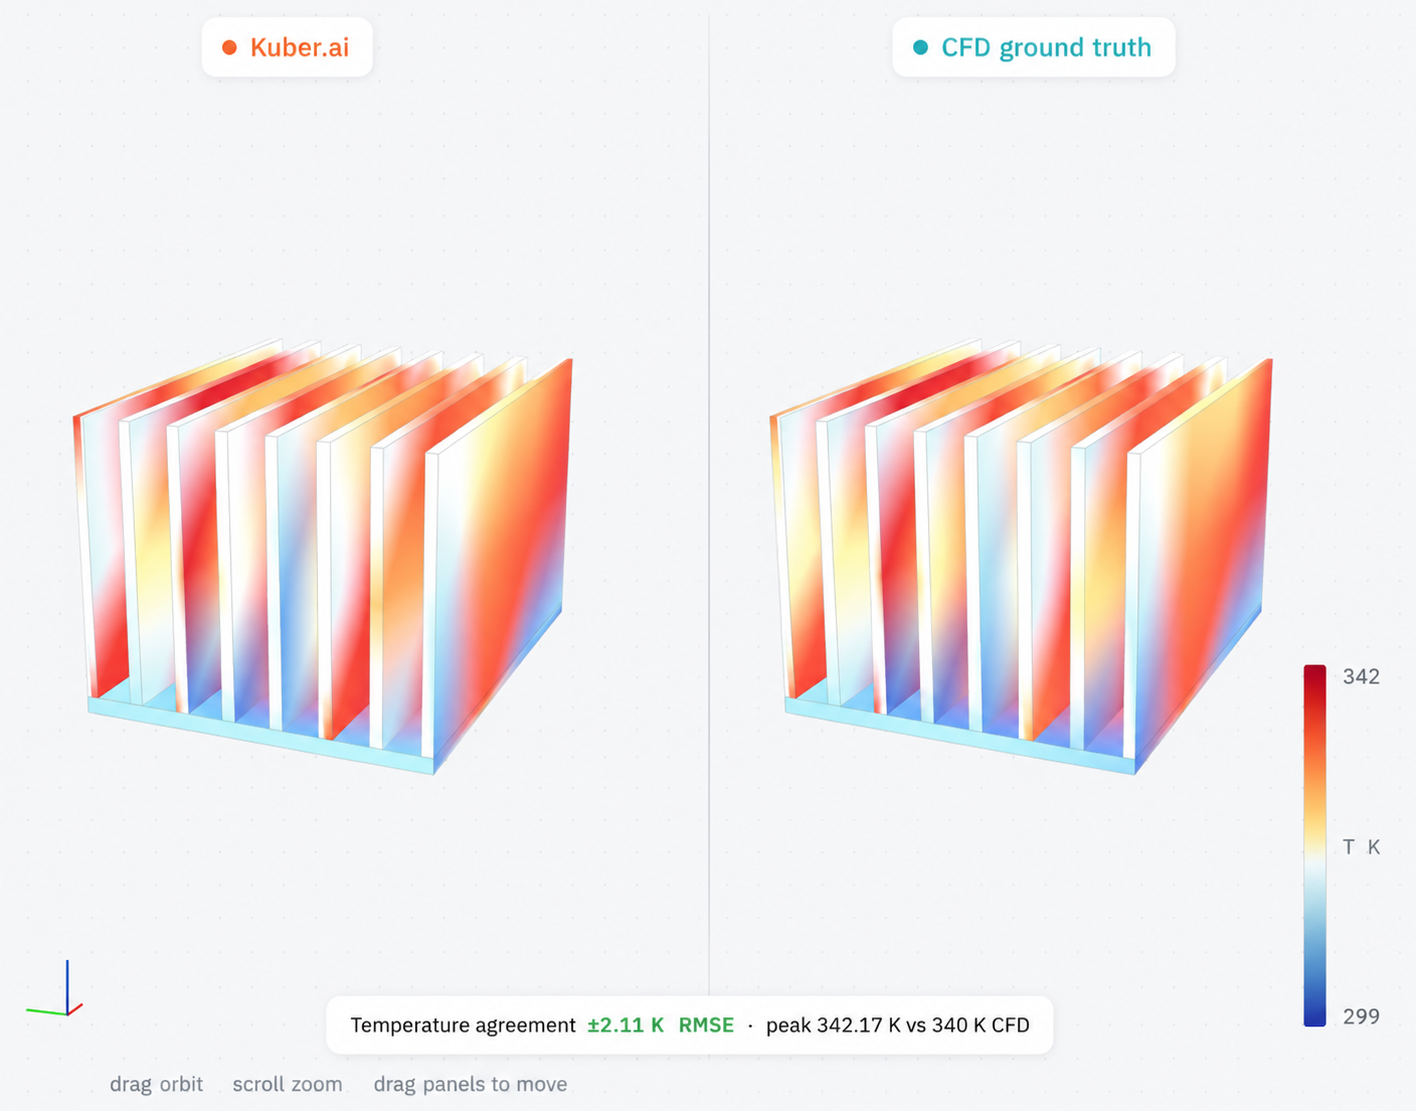
\includegraphics[width=0.72\textwidth]{heat-sink-comparison.png}
\caption{Kuber prediction vs. CFD ground truth for a heatsink simulation: surface temperature field on
the finned solid, $\pm$2.11\,K RMSE agreement (peak 342.17 vs.\ 340\,K CFD), computed 7{,}000$\times$
faster than the CFD solver.}
\label{fig:hero}
\end{figure*}

\section{Related Work}
\textit{Neural operators.} DeepONet~\cite{deeponet} and the Fourier Neural Operator~\cite{fno}
established learning maps between function spaces; GINO~\cite{gino} extended operator learning to
large 3D geometries. These are strong on fixed domains but do not natively consume arbitrary boundary
geometry with per-node queries. \textit{Transformer PDE (partial-differential-equation) solvers.} Transolver~\cite{transolver}
introduced physics attention over learned slices; UPT~\cite{upt} and the anchored/branched
variant~\cite{abupt} scale transformer surrogates to industrial CFD. Our core builds on the
GeoTransolver implementation in NVIDIA PhysicsNeMo~\cite{physicsnemo}; our contribution is the
surface-conditioning branch and the CHT-specific conditioning and training recipe.
\textit{Geometry representations.} Signed-distance fields (SDFs) are data-efficient when an analytic shape
exists, but none exists for arbitrary CAD (computer-aided-design geometry); following the surface branch of AB-UPT~\cite{abupt} we
encode the boundary directly as a point cloud with normals. \textit{Spectral fidelity.} One-shot
regression is spectrally biased; PDE-Refiner~\cite{pderefiner} restores high-frequency content, which
we adopt as an optional head. \textit{Benchmarks.} SIMSHIFT~\cite{simshift} is a public benchmark for
distribution shift in engineering simulation; we use its heatsink task as our primary evaluation.

\section{Problem Formulation}
A CHT case consists of a solid conductor with boundary $\Gamma$ immersed in a fluid domain $\Omega$.
Given the boundary geometry and operating conditions, we seek the steady field at any query point
$x\in\Omega$:
\begin{equation}
f_\theta:\ (x,\ \Gamma,\ c)\ \mapsto\ (U_x,U_y,U_z,T,p_{\mathrm{rgh}}),
\end{equation}
where $U$ is velocity, $T$ temperature, and $p_{\mathrm{rgh}}=p-\rho g h$ the reduced pressure. The
conditioning vector $c$ collects fluid properties (Prandtl number, density, specific heat, dynamic
viscosity), boundary conditions (BCs; a wall temperature for heatsinks or a heat flux for cold plates, and
the ambient/inlet temperature), inlet velocity, and a binary device-class flag. The boundary $\Gamma$
is presented as surface points with outward unit normals. Nothing in the input assumes a parametric
shape family.

\section{Method}\label{sec:method}
\subsection{KuberNet}
A \textbf{surface encoder} maps the boundary point cloud with normals to permutation-invariant
geometry tokens via a shallow self-attention stack. A \textbf{local cross-attention} module produces,
for every query node, a geometry descriptor by attending over its $k{=}16$ nearest surface tokens, so
each query carries a local view of the nearby boundary. This descriptor is concatenated with the
broadcast conditioning vector to form the per-node embedding. The \textbf{core} is a GeoTransolver
physics-attention transformer (256 hidden units, 12 layers, 8 heads, 64 physics slices, with
multiscale local ball-query features) that regresses the five $z$-normalized (standardized: zero mean, unit variance) targets. The model has
approximately 14.3\,M parameters. A PDE-Refiner head refines the one-shot
regression (detailed below). Geometry may alternatively be supplied as a
(directional) signed-distance field for parametric families, but the surface-encoder configuration is
the one we report because it is the only one applicable to arbitrary CAD.

Formally, write the surface as points $p_i\in\mathbb{R}^3$ with unit normals $n_i$ ($i{=}1{\dots}N_s$),
the query cloud as $x_j$ ($j{=}1{\dots}N$), and the conditioning as $c\in\mathbb{R}^C$. The surface
encoder embeds each element with a multi-layer perceptron (MLP) and applies an $L_s$-layer pre-norm Transformer with multi-head
self-attention (MHSA):
\begin{equation}
h_i^0=\mathrm{MLP}([p_i;n_i]),\ \ H\!\leftarrow\!H+\mathrm{MHSA}(\mathrm{LN}\,H),\ \ H\!\leftarrow\!H+\mathrm{FFN}(\mathrm{LN}\,H),
\end{equation}
with $\mathrm{MHSA}(Q,K,V)=\mathrm{softmax}(QK^\top/\sqrt{d})V$, yielding geometry tokens $z_i=H_i^{(L_s)}$.
For each query $x_j$, let $\mathcal{N}_k(j)$ be its $k$ nearest surface points (k-nearest neighbors, kNN); with relative positions
$r_{ji}=x_j-p_i$, learned bias $b_{ji}=\mathrm{MLP}_r(r_{ji})$, and query $q_j=\mathrm{MLP}_q(x_j)$, the
local geometry descriptor is
\begin{equation}
\alpha_{ji}=\operatorname*{softmax}_{i\in\mathcal{N}_k(j)}\Big(\frac{q_j^\top(W_K z_i+b_{ji})}{\sqrt{d_h}}-\gamma\,|r_{ji}\!\cdot\!n_i|\Big),\qquad
g_j=W_O\!\!\sum_{i\in\mathcal{N}_k(j)}\!\!\alpha_{ji}\,(W_V z_i+b_{ji}),
\end{equation}
(multi-head; heads omitted). The penalty $-\gamma\,|r_{ji}\!\cdot\!n_i|$ is \emph{Anisotropic
Boundary-Layer} (ABL) attention: it down-weights the wall-normal component of the query-to-node
displacement (learned $\gamma=\mathrm{softplus}(\cdot)\ge 0$, with $\gamma=0$ recovering isotropic kNN),
so a query inside a thin thermal boundary layer attends \emph{along} the wall rather than across it---the
anisotropy that plain Euclidean distance ignores, and (Sec.~\ref{sec:ablation}) our largest single accuracy
gain. Locality and relative positions make $g_j$ compositional---a 10-fin heatsink is locally ``more of the
same'' fin-gap patches seen at 5--8 fins. The per-node embedding
$e_j=[g_j;c]$ is lifted, $u_j^0=\mathrm{MLP}([e_j;x_j])$, and passed through $L_c$ \emph{physics-attention}
blocks. Each block softly assigns the $N$ nodes to $M$ learned slices, aggregates them into slice tokens,
attends among the tokens, and scatters back:
\begin{equation}
w_{jm}=\operatorname*{softmax}_m(u_j^\top\theta_m),\quad
t_m=\frac{\sum_j w_{jm}u_j}{\sum_j w_{jm}},\quad
u_j\leftarrow u_j+\sum_m w_{jm}\,\mathrm{MHSA}(T)_m,
\end{equation}
followed by a multiscale ball-query aggregation at radii $\{0.05,0.25\}$ and an FFN, each with a residual
and LN; the slice mechanism costs $O(NM)$ with $M\ll N$ instead of the $O(N^2)$ of dense attention. A
linear head gives the $z$-normalized field, trained by mean-squared error and de-normalized to physical
units:
\begin{equation}
\hat{y}_j=W_o u_j^{(L_c)}\in\mathbb{R}^5,\quad
\mathcal{L}(\theta)=\frac{1}{BN}\sum_{b,j}\lVert\hat{y}_{bj}-y_{bj}\rVert^2,\quad
\text{field}=\hat{y}_j\odot\sigma_y+\mu_y.
\end{equation}
Here $N_s$ and $N$ are the numbers of surface and query points and $C$ the number of conditioning
scalars; $L_s,L_c$ the encoder and core depths and $M$ the slice count; $d,d_h$ the model and per-head
attention widths and $d_s,d_g$ the token and descriptor widths; $Q,K,V$ the attention query/key/value
matrices; $W_K,W_V,W_O,W_o$ learned projection matrices and $\theta_m$ the $M$ learned slice queries;
$\sigma_y,\mu_y$ the per-channel target standard deviation and mean, $\odot$ the elementwise product, $B$
the batch size, and $\theta$ all trainable parameters. Every MLP is two-layer with a GELU activation;
FFN denotes a feed-forward network and LN layer normalization.

\begin{figure*}[t]
\centering
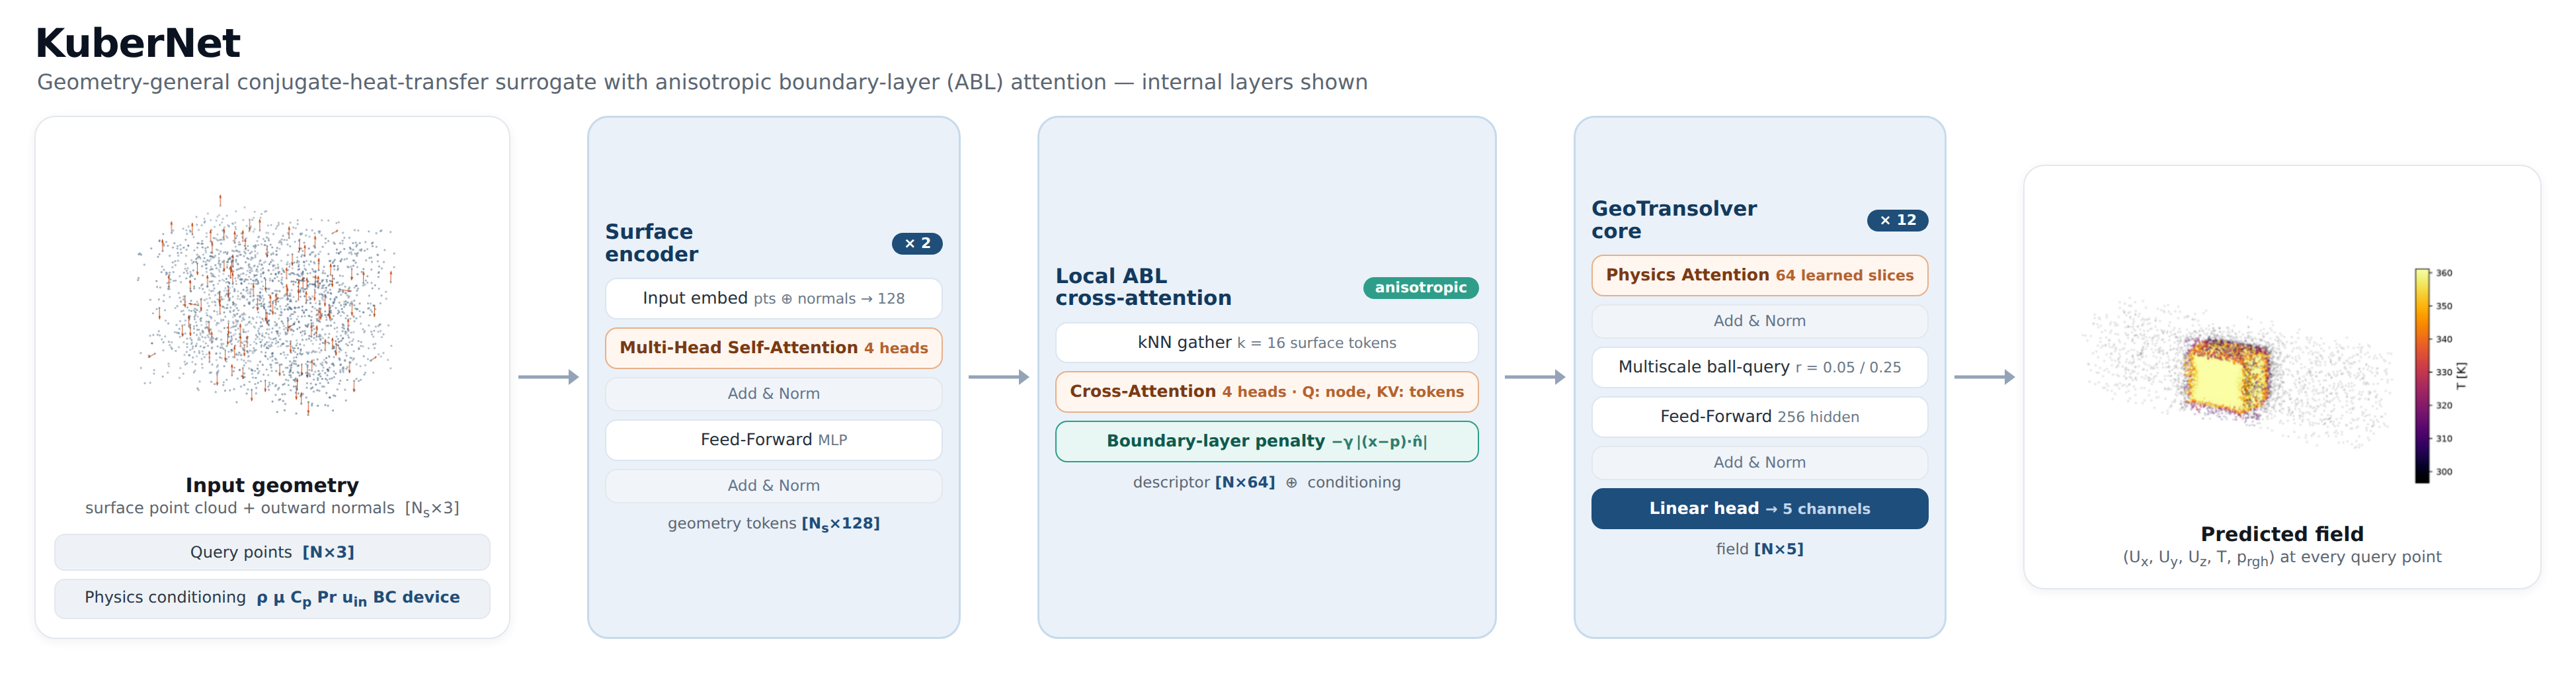
\includegraphics[width=0.96\textwidth]{architecture.png}
\caption{KuberNet. Three inputs---the boundary surface point cloud with normals, the query
points, and the physics conditioning---feed a neural spine (surface encoder $\rightarrow$ local
anisotropic boundary-layer (ABL) cross-attention $\rightarrow$ concatenated per-node embedding $\rightarrow$ GeoTransolver
physics-attention core) that predicts the five-channel field at every query node.}
\label{fig:arch}
\end{figure*}

\subsection{PDE-Refiner Head}
\textit{Why we use it.} One-shot regression under a mean-squared-error loss is \emph{spectrally biased}:
low-amplitude high-frequency modes---sharp fin-tip gradients, thin thermal boundary layers---contribute
little to the squared error, so a single forward pass tends to over-smooth them. PDE-Refiner~\cite{pderefiner}
removes this bias by casting field prediction as an iterative \emph{denoising} process, whose training
objective forces the network to represent structure at every spatial frequency; as a by-product,
sampling the noise yields an ensemble and hence an uncertainty estimate.

\textit{How we use it.} The same network $f_\theta$ serves as both the signal predictor and the
denoiser, conditioned on a refinement step $k\in\{0,\dots,K\}$ through a sinusoidal step embedding and an
extra noised-field input channel. With a geometric noise schedule $\sigma_k=\sigma_{\min}^{\,k/K}$
($\sigma_0=0$), each training sample draws $k\sim\mathrm{Uniform}\{0,\dots,K\}$: at $k{=}0$ the network
regresses the field $y$ from the conditioning; at $k\ge1$ it is given the target corrupted by noise,
$y+\sigma_k\epsilon$ ($\epsilon\sim\mathcal{N}(0,I)$), and regresses the noise $\epsilon$. At inference we
take the initial one-shot prediction and apply $K$ refinement steps,
\begin{equation}
u\leftarrow f_\theta(\cdot,0);\quad k{=}1{\dots}K:\ \ u\leftarrow(u+\sigma_k\epsilon)-\sigma_k\,f_\theta(u+\sigma_k\epsilon,\,k),
\end{equation}
so each step subtracts the network's predicted noise and restores fine structure; drawing several noise
seeds $\epsilon$ gives an ensemble whose spread is a calibrated uncertainty. The refiner is the
framework's spectral-fidelity head: it recovers the sharp near-wall temperature gradients that a one-shot
mean-squared-error fit over-smooths. The out-of-distribution accuracy in Sec.~V is reported from the
one-shot model ($k{=}0$); the refiner is the mechanism we apply when near-wall gradient fidelity or
calibrated uncertainty is the priority, and it seeds the Uncertainty pillar of the suite.

\subsection{Data Engine}
We generate CHT data with OpenFOAM's steady buoyant solver (\texttt{buoyantSimpleFoam}) over a single
fluid region, treating the solid as a heated wall (heatsinks) or heat-flux surface (cold plates). A
parametric generator samples geometry and conditions; the geometry is meshed with \texttt{blockMesh}
and \texttt{snappyHexMesh} plus prism layers, solved, and exported to 16{,}384 fluid nodes with the
five field channels, the boundary surface cloud with normals, and a JSON of conditions. The pipeline
is resumable and gated: a case is written only after a converged solve, and a physics filter rejects
unphysical results. Sampling is seeded, so the corpus regenerates deterministically. It is entirely
self-generated (Table~\ref{tab:corpus}).

\begin{table}[t]\renewcommand{\arraystretch}{1.15}
\caption{Data-Engine Coverage of the Self-Generated Corpus}
\label{tab:corpus}\centering
\begin{tabular}{@{}ll@{}}\toprule
Axis & Coverage \\ \midrule
Fluids & air, water, oil (Pr$\approx$292), glycol \\
Regimes & natural + forced convection \\
Shapes & fins, plate, cube, pin-fin; duct channels \\
Devices & heatsink (wall-$T$), cold plate (heat-flux) \\
Fidelity & $\approx$1.4\,M cells/case $\rightarrow$ 16{,}384 nodes \\ \bottomrule
\end{tabular}
\end{table}

\section{Experimental Setup}
\textit{Benchmark.} Our primary, externally comparable evaluation is the SIMSHIFT~\cite{simshift}
heatsink task at \emph{medium} difficulty: train on fin counts 5--8, test on the shifted, out-of-distribution (OOD) target of fin
counts 10--12, which never appear in training. We train from scratch on the 222 training cases;
normalizers are fit on the source training split only. \textit{Metrics.} We report per-field root-mean-square error (RMSE) in
physical units and normalized RMSE (nRMSE); the benchmark's primary selector is mean nRMSE across the
five fields. We additionally report near-wall $T$-RMSE and edge gradient ratios (Sec.~\ref{sec:stab}).
No baseline uses \emph{unsupervised domain adaptation} (UDA)---training-time adaptation to the
\emph{unlabeled} target (test) distribution, e.g.\ aligning source- and target-domain feature
statistics to shrink the out-of-distribution gap---in our runs; the published baselines do, which
is their best case. \textit{Training.} Adam~\cite{adam} at learning rate $10^{-3}$, batch size 4 cases
(16{,}384 query nodes each), with a warmup--stable--decay schedule: a 5-epoch linear warmup, a stable
phase held until the validation mean-nRMSE plateaus (patience 25 epochs), then a 30-epoch cosine decay
to $10^{-6}$; the best-validation checkpoint is kept. Targets are $z$-scored per channel and coordinates
mapped to a per-case unit frame. The encoder uses $d_s{=}128$ (2 layers, 4 heads); the descriptor
$d_g{=}64$ with $k{=}16$; the core is 256-wide, 12 layers, 8 heads, $M{=}64$ slices, ball-query radii
$\{0.05,0.25\}$ with $\{8,32\}$ neighbors ($\approx$14.3\,M parameters). Baseline numbers are quoted from
the SIMSHIFT paper.

\section{Results}
\subsection{SIMSHIFT Heatsink Benchmark}
On temperature---the design-critical field---KuberNet improves on the best previously
published result while using no UDA (Table~\ref{tab:lead}). The paper reports only temperature and
velocity RMSE on the target domain; baseline parameter counts are not published but their released
configurations are comparably sized ($\sim$10--15\,M), so the improvement is not from scale.

\begin{table}[t]\renewcommand{\arraystretch}{1.2}
\caption{SIMSHIFT Heatsink, Medium (OOD) Split. Baselines Include UDA; Ours Does Not. Lower is Better.}
\label{tab:lead}\centering
\begin{tabular}{@{}lccc@{}}\toprule
Model & UDA & Temp RMSE (K) & mean nRMSE \\ \midrule
\textbf{KuberNet} (ours) & \ding{55} & \textbf{11.84} & \textbf{0.608} \\
UPT (prev. best)~\cite{upt} & \ding{51} & 12.41 & --- \\
Transolver~\cite{transolver} & \ding{51} & 13.43 & --- \\
PointNet~\cite{pointnet} & \ding{51} & 17.43 & --- \\ \bottomrule
\end{tabular}
\end{table}

KuberNet attains \textbf{11.84\,K} temperature RMSE and \textbf{0.608} mean nRMSE (our primary selector) on
the medium out-of-distribution split, beating the previous published best (UPT, 12.41\,K) with no domain
adaptation. The gain is driven by its \emph{anisotropic boundary-layer} attention (Sec.~\ref{sec:method}):
ablating it to isotropic kNN raises error to 12.14\,K / 0.671---a 9\% larger mean nRMSE at equal parameter
count (Sec.~\ref{sec:ablation}). The comparison to prior work is like-for-like: the SIMSHIFT baselines are
also conditioned on geometry and operating scalars (they report temperature only, so mean nRMSE is dashed)
and additionally use UDA, which we do not; these are single-run numbers, with multi-seed replicates in progress.
The benchmark number is itself out of distribution---Table~\ref{tab:srctgt} separates in-distribution
accuracy (3.96\,K) from the shifted target.

\begin{table}[t]\renewcommand{\arraystretch}{1.2}
\caption{KuberNet: Source (In-Distribution) vs. Target (OOD) Detail}
\label{tab:srctgt}\centering
\begin{tabular}{@{}lcccc@{}}\toprule
Domain & $T$ (K) & near-wall $T$ & $p_{\mathrm{rgh}}$ & mean nRMSE \\ \midrule
source (in-dist.) & 3.96 & 2.80 & 202 & 0.274 \\
target (OOD) & 11.84 & 11.35 & 2305 & 0.608 \\ \bottomrule
\end{tabular}
\end{table}

\subsection{One Model, Two Device Classes}
A single set of weights, distinguished only by the device flag and fluid/BC conditioning, spans a
wall-temperature, buoyancy-driven heatsink in air and a heat-flux, forced-liquid cold plate. Evaluated
per class on held-out cases from our corpus (there is no public cold-plate CHT benchmark), the model
reaches the errors in Table~\ref{tab:multi}. The cold-plate mean nRMSE (0.028) is close to the
in-distribution value. These numbers are on our own corpus and are not comparable to the SIMSHIFT
numbers.

\begin{table}[t]\renewcommand{\arraystretch}{1.2}
\caption{Multi-Geometry Model, Held Out per Device Class (Our Corpus)}
\label{tab:multi}\centering
\begin{tabular}{@{}lccc@{}}\toprule
Held-out class & $T$ RMSE (K) & $T$ nRMSE & mean nRMSE \\ \midrule
cold plates & 3.11 & 0.039 & 0.028 \\
heatsinks & 5.13 & 0.065 & 0.145 \\
in-distribution (both) & 1.72 & 0.022 & 0.027 \\ \bottomrule
\end{tabular}
\end{table}

\begin{figure*}[t]
\centering
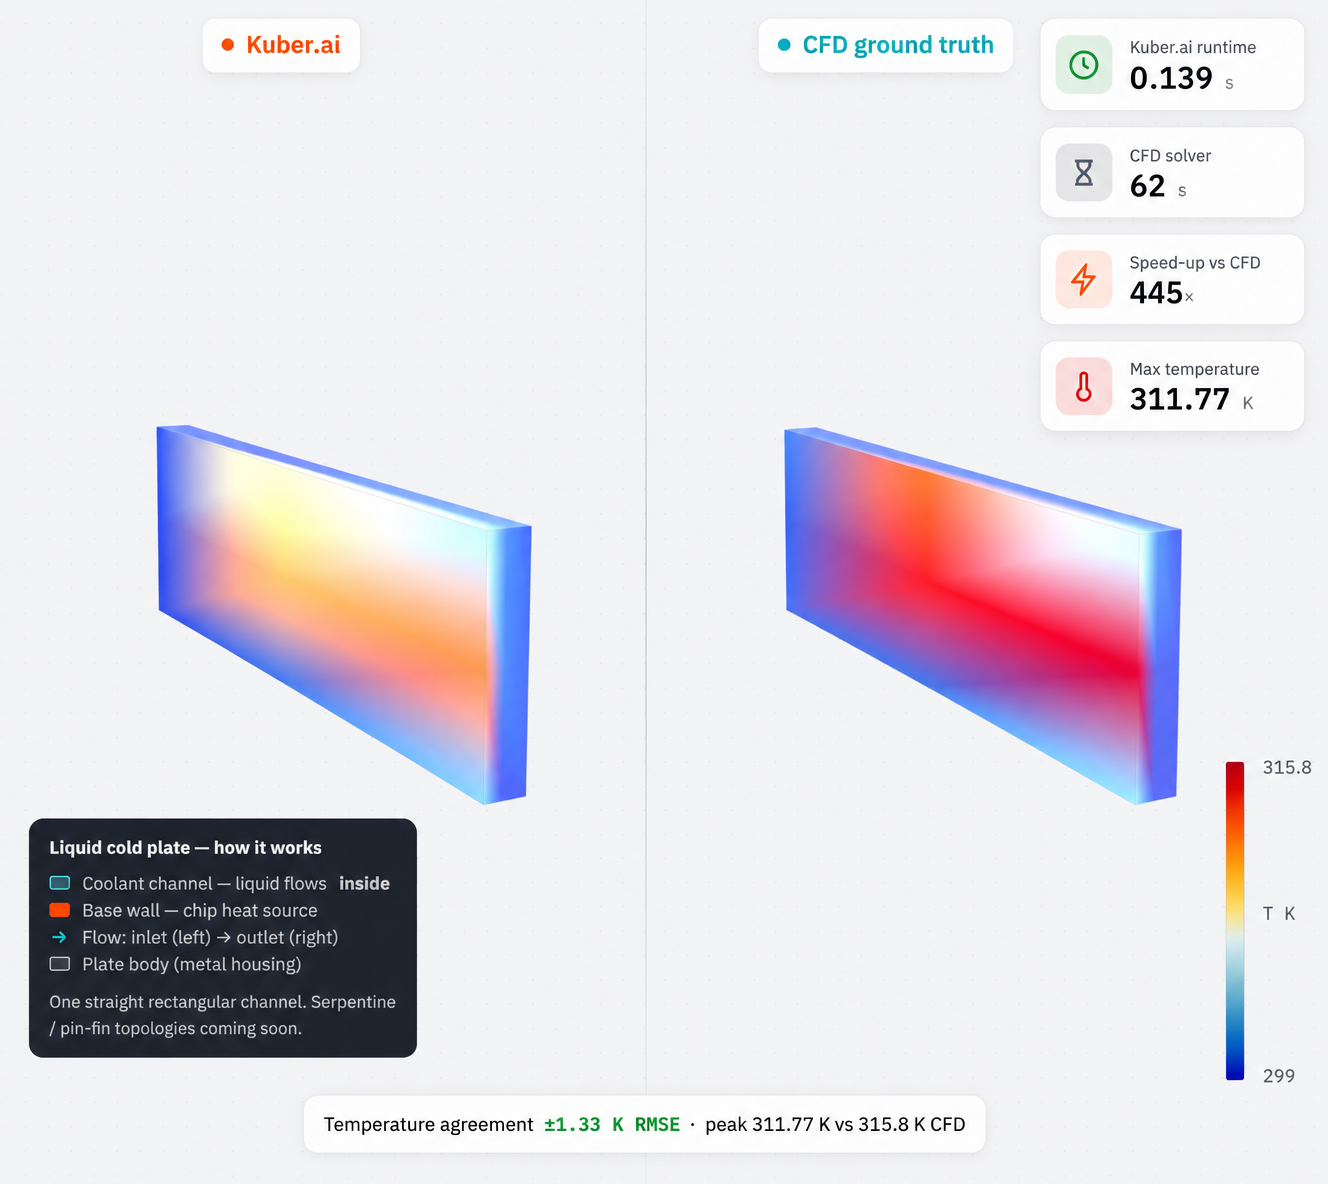
\includegraphics[width=0.70\textwidth]{cold-plate-comparison.png}
\caption{Kuber prediction vs. CFD ground truth for a liquid cold-plate simulation: surface temperature
field, $\pm$1.33\,K RMSE agreement (peak 311.77 vs.\ 315.8\,K CFD), computed 445$\times$ faster than the CFD solver.}
\label{fig:gtpred}
\end{figure*}

\subsection{Pretraining and Reduced Conditioning}
The headline results (Tables~\ref{tab:lead}--\ref{tab:srctgt}) condition on the same twelve
geometry/physics scalars that Transolver and the other baselines receive, for a like-for-like comparison.
We now isolate two orthogonal levers that trade explicit scalars for learned priors: \emph{pretraining} on
the self-generated corpus, and \emph{reduced conditioning}---dropping the geometry scalars and keeping only
the wall temperature---which together point toward a geometry-and-physics foundation model. First, does
pretraining help beyond the benchmark's own training set? A controlled A/B with the same model and SIMSHIFT
fine-tuning, changing only the initialization (Table~\ref{tab:vod}). Pretraining helps materially at the
easy shift ($-19\%$) and in-distribution ($-12\%$), modestly at medium, and is neutral at the hardest
shift, which the corpus does not yet cover. The only changed ingredient is the corpus.

\begin{table}[t]\renewcommand{\arraystretch}{1.2}
\caption{Temperature RMSE (K); From Scratch vs. Corpus-Pretrained Then Fine-Tuned}
\label{tab:vod}\centering
\begin{tabular}{@{}lccc@{}}\toprule
Shift & from scratch & pretrained & $\Delta$ \\ \midrule
easy & 8.99 & \textbf{7.28} & $-19\%$ \\
medium & 12.94 & \textbf{12.38} & $-4.3\%$ \\
hard & 14.42 & 14.43 & $\pm 0$ \\
in-dist. & 4.63 & \textbf{4.09} & $-12\%$ \\ \bottomrule
\end{tabular}
\end{table}

\textbf{Why it helps, and why it is not leakage.} With only a few hundred fine-tuning cases,
initialization matters: pretraining on the broader OpenFOAM corpus supplies a physics prior---the
coupling of temperature and flow, near-wall behavior, and boundary-layer structure---that is hard to
learn from the small target set alone, which is why the gain is largest at the easy shift and
in-distribution and tapers at the hardest shift the corpus does not cover. Critically, \emph{no
held-out evaluation data is ever seen during pretraining or fine-tuning}: the pretraining corpus is our
own OpenFOAM data, disjoint from the SIMSHIFT benchmark and its splits; the SIMSHIFT target
(out-of-distribution) split is used only for evaluation; and in the multi-geometry setting the held-out
per-device cases are excluded from training. The gains reflect transfer of physics, not exposure to
the test distribution.

\textbf{Toward a reduced-conditioning foundation model.} The two levers compose. Dropping the geometry
scalars alone raises medium-shift error from 12.14 to 12.94\,K (Table~\ref{tab:abl})---the model must now
read fin count and gap from the point cloud rather than from a scalar---but corpus pretraining recovers most
of that gap ($12.94\!\to\!12.38$\,K), so a model told almost nothing about the geometry beyond its shape
nearly matches the fully-conditioned one. To make the little conditioning it does keep transferable across
working fluids, we replace raw fluid properties with Buckingham-$\Pi$ dimensionless groups
($\mathrm{Re},\mathrm{Ra},\mathrm{Pe}$, appended in log-space; $\mathrm{Pr}$ is already a channel), so air,
water, and oil map to a common similarity space rather than disjoint property ranges. Pretraining this
$\Pi$-conditioned, geometry-scalar-free model on the full multi-geometry corpus and fine-tuning on SIMSHIFT
is the foundation-model arm; that run is in progress and its numbers will be reported in the camera-ready.
The direction matters because a surrogate that infers behavior from shape and dimensionless physics---not
from a fixed scalar template---is the one that generalizes to geometries and fluids outside any benchmark's
schema.

\subsection{Numerical Stability}\label{sec:stab}
A deployable surrogate must reproduce steep near-wall gradients without over-smoothing or emitting
unphysical spikes. We measure the ratio of predicted to CFD temperature-gradient magnitude in the edge
band and at the steepest peaks (Table~\ref{tab:stab}). Every ratio is at or below unity, in and out of
distribution---the surrogate never produces a steeper-than-physical gradient---with an explosion
fraction of exactly zero and no NaN/Inf. It is not merely over-smoothing: the in-distribution edge
ratio ($0.97\approx1.0$) reproduces the true edge structure, while out of distribution it errs
slightly conservative, the safe direction.

\begin{table}[t]\renewcommand{\arraystretch}{1.2}
\caption{Predicted/CFD Temperature-Gradient Ratio at Edges (1.0 = Faithful)}
\label{tab:stab}\centering
\begin{tabular}{@{}lcc@{}}\toprule
Metric & in-dist. & OOD \\ \midrule
edge-band $\nabla T$ ratio & 0.969 & 0.746 \\
steepest-peak (p99.9) ratio & 0.938 & 0.725 \\
explosion fraction & 0 & 0 \\
NaN / Inf count & 0 & 0 \\ \bottomrule
\end{tabular}
\end{table}

\subsection{Speed and Data Fidelity}
Inference is a single forward pass whose cost is independent of geometry, unlike CFD whose cost grows
with mesh size. Against measured OpenFOAM solve times (median 22 minutes, up to 117 for fine
geometries), a sub-second forward pass is up to four orders of magnitude ($\approx$10,000$\times$)
faster; we report the inference figure as an estimate pending exact per-GPU timing. On fidelity, three prism boundary
layers recover the near-wall hot spot to within 0.1\,K of a fine mesh (378.8 vs.\ 378.9\,K) at
$\approx$2.7$\times$ fewer cells.

\subsection{Ablations}\label{sec:ablation}
Table~\ref{tab:abl} isolates the main design choices on the SIMSHIFT medium split. \textbf{Every row changes
exactly one factor and holds the rest of the 14.3M-parameter backbone fixed}, so the gap between the
\emph{base} column (the reference that ablation was measured against) and the \emph{result} column is that
factor's isolated effect. The attention and output-head rows are measured against the full KuberNet reference
(11.84\,K); the geometry, conditioning, and pretraining rows---established before ABL was added---are measured
against the isotropic-kNN configuration (12.14\,K, i.e.\ the ``remove ABL'' row), and pretraining against its
from-scratch reduced-conditioning baseline (12.94\,K). Reading the effects: \textbf{anisotropic boundary-layer
attention is KuberNet's largest single design win}---removing it costs 0.30\,K ($11.84\!\to\!12.14$, mean nRMSE
$0.608\!\to\!0.671$) at equal parameter count. Adding a PDE-Refiner head is fine in-distribution (4.15\,K) but
degrades OOD to 16.52\,K---its iterative refinement amplifies error under distribution shift---which is why we
report the one-shot model. The surface encoder, unlike the analytic SDF, applies to arbitrary CAD; the SDF
variant is data-efficient (lower averaged nRMSE, 0.593, and velocity, 0.038\,m/s) but presupposes an analytic
shape. Full 12-scalar conditioning improves temperature by 0.8\,K over wall-temperature-only, confirming the
fluid-property and boundary-condition scalars carry signal, and corpus pretraining recovers 0.56\,K of that
reduced setting ($12.94\!\to\!12.38$\,K). Both the full-conditioning and pretrained models pass UPT's
12.41\,K. Separately, feeding the surface as a per-node descriptor (used here) generalized better than
AB-UPT-style per-block cross-attention on the raw surface cloud at this data scale.

\begin{table}[t]\renewcommand{\arraystretch}{1.2}
\caption{KuberNet ablations on SIMSHIFT Medium (OOD). Each row changes one factor from a fixed reference; ``base'' is that reference's error, ``result'' the ablated model's. Temperature RMSE (K), lower is better.}
\label{tab:abl}\centering
\begin{tabular}{@{}l p{3.2cm} c c@{}}\toprule
Factor & One change from reference & base & result \\ \midrule
reference & \textbf{KuberNet}: ABL, surf.\ enc., 12 scalars, one-shot head & --- & \textbf{11.84} \\
attention & remove ABL $\to$ isotropic kNN & 11.84 & 12.14 \\
output head & add PDE-Refiner & 11.84 & 16.52 \\
geometry input & surface encoder $\to$ analytic SDF & 12.14 & 13.07 \\
conditioning & 12 scalars $\to$ wall-$T$ only & 12.14 & 12.94 \\
pretraining & add corpus pretrain (wall-$T$ cond.) & 12.94 & \textbf{12.38} \\ \bottomrule
\end{tabular}
\end{table}

\section{Discussion and Limitations}
We state the boundaries plainly. The corpus is air-dominated (tens of oil/glycol cases), so the model
is strongest on air. On SIMSHIFT the OOD axis is fin count alone; leave-one-fluid-out and
leave-one-shape-out remain future work. Cold plates are currently straight-channel, so the
multi-geometry result shows device-class generality rather than topology extrapolation. On the
averaged-nRMSE selector our temperature lead is bought with slightly higher velocity and pressure
error, reported transparently. Inference latency is an estimate. The multi-geometry numbers are on our
own corpus and are not comparable to the public benchmark.

\textit{Future work.} ABL attention (Sec.~\ref{sec:method}) and Buckingham-$\Pi$ conditioning with corpus
pretraining (Sec.~\ref{sec:ablation}) are realized in the present model; the directions below remain, each
stated with its rationale so results can be filled in as runs complete. \textbf{(i)~Leave-One-Fluid-Out
(LOFO):} train on air and water and evaluate zero-shot on high-viscosity oil ($\mathrm{Pr}\approx292$), a
stronger out-of-distribution axis than fin count. \textbf{(ii)~Interface flux-balanced loss:} a soft residual
enforcing conjugate energy conservation, $k_s(\nabla T_s\!\cdot\!\mathbf{n})=k_f(\nabla T_f\!\cdot\!\mathbf{n})$,
at solid--fluid interfaces; this requires two-region (conjugate) training data that our current
single-region corpus does not provide, so it is paired with a data-engine extension.
\textbf{(iii)~Physics-masked pretraining:} a self-supervised objective reconstructing masked spatial regions
and physical channels (e.g.\ predicting $T$ from $U$ and geometry), forcing the backbone to internalize
conservation and improving data efficiency. Alongside these, scaling model and corpus (the value-of-data
trend favors both), hierarchical surface tokens, calibrated uncertainty from the refinement head, further
cold-plate topologies, and ONNX/TensorRT deployment within an agentic propose--predict--score--refine
optimization loop with CAD connectors (STEP/STL/mesh) remain on the roadmap.

\section{Conclusion}
Kuber packages the full stack needed to build a CHT surrogate---a reproducible data engine, an honest
evaluation harness, and \textbf{KuberNet}, a geometry-general surface-conditioned transformer whose
anisotropic boundary-layer attention reaches state of the art (11.84\,K temperature RMSE) on a public
benchmark without domain adaptation and spans two device classes from one set of weights. The same interfaces target the broader class of
coupled fluid--heat problems. Calibrated uncertainty, CAD connectors, and agentic geometry optimization
are natural next steps; code, data, and an interactive viewer are released to support them.

\begin{thebibliography}{00}
\bibitem{pointnet} C.~R. Qi, H.~Su, K.~Mo, and L.~J. Guibas, ``PointNet: Deep learning on point sets for 3D classification and segmentation,'' in \emph{Proc. IEEE CVPR}, 2017.
\bibitem{simshift} P.~Setinek \emph{et al.}, ``SIMSHIFT: A benchmark for distribution shift in engineering simulation,'' preprint, 2025.
\bibitem{transolver} H.~Wu, H.~Luo, H.~Wang, J.~Wang, and M.~Long, ``Transolver: A fast transformer solver for PDEs on general geometries,'' in \emph{Proc. ICML}, 2024.
\bibitem{upt} B.~Alkin, A.~F\"urst, S.~Schmid, L.~Gruber, M.~Holzleitner, and J.~Brandstetter, ``Universal physics transformers,'' in \emph{Proc. NeurIPS}, 2024.
\bibitem{abupt} B.~Alkin \emph{et al.}, ``Anchored/branched universal physics transformers,'' preprint, 2025.
\bibitem{fno} Z.~Li \emph{et al.}, ``Fourier neural operator for parametric partial differential equations,'' in \emph{Proc. ICLR}, 2021.
\bibitem{deeponet} L.~Lu, P.~Jin, G.~Pang, Z.~Zhang, and G.~E. Karniadakis, ``Learning nonlinear operators via DeepONet,'' \emph{Nature Machine Intelligence}, 2021.
\bibitem{gino} Z.~Li \emph{et al.}, ``Geometry-informed neural operator for large-scale 3D PDEs,'' in \emph{Proc. NeurIPS}, 2023.
\bibitem{pderefiner} P.~Lippe, B.~Veeling, P.~Perdikaris, R.~Turner, and J.~Brandstetter, ``PDE-Refiner: Achieving accurate long rollouts with neural PDE solvers,'' in \emph{Proc. NeurIPS}, 2023.
\bibitem{physicsnemo} NVIDIA, ``PhysicsNeMo: A framework for physics-ML (GeoTransolver),'' software, Apache-2.0.
\bibitem{adam} D.~P. Kingma and J.~Ba, ``Adam: A method for stochastic optimization,'' in \emph{Proc. ICLR}, 2015.
\bibitem{weller} H.~G. Weller, G.~Tabor, H.~Jasak, and C.~Fureby, ``A tensorial approach to computational continuum mechanics using object-oriented techniques,'' \emph{Computers in Physics}, vol.~12, no.~6, 1998.
\end{thebibliography}

\end{document}
